
\documentclass[12pt,a4paper]{article} 

\usepackage{float,times,graphicx,mathtools}
\usepackage{amsmath}
\usepackage{amsfonts}
\usepackage{amssymb}
\usepackage{latexsym}
\usepackage{epsfig}
\usepackage{graphicx}
\usepackage{caption}
\usepackage{subcaption}
\usepackage{color}
\usepackage{pdfpages}
\usepackage{natbib}
\usepackage[space]{grffile}
\usepackage{wrapfig}
\usepackage{subcaption}
\usepackage{url}
\usepackage{bbm}
\usepackage{tikzsymbols}

\DeclareMathOperator{\logit}{logit}
\DeclareMathOperator{\tr}{tr}
\bibpunct[, ]{(}{)}{;}{a}{,}{,}
\graphicspath{{../}}  
\addtolength{\oddsidemargin}{-1in}
	\addtolength{\evensidemargin}{-1in}
	\addtolength{\textwidth}{1.75in}
	\addtolength{\topmargin}{-1.3in}
	\addtolength{\textheight}{2in}
\date{\vspace{-5ex}}
\begin{document}

\begin{itemize}
\item Pulled in population data for Burkina Faso 
\begin{itemize}
\item[--] Allowed a different hypervariance for the WPP baseline
\item[--] Estimated child mortality and fertility rates oscillates around the initial estimates, possibly due to the previously mentioned under-count in young age groups
\item[--] Excluded age group 0-4 from the likelihood, problem still persists
\item[--] Excluded the first two age groups (0-4, 5-9) and it is fine
\item[--] Estimated correlation in migration proportions across time is negative \Changey[1.5]{-1}
\end{itemize}
\item 

\end{itemize}

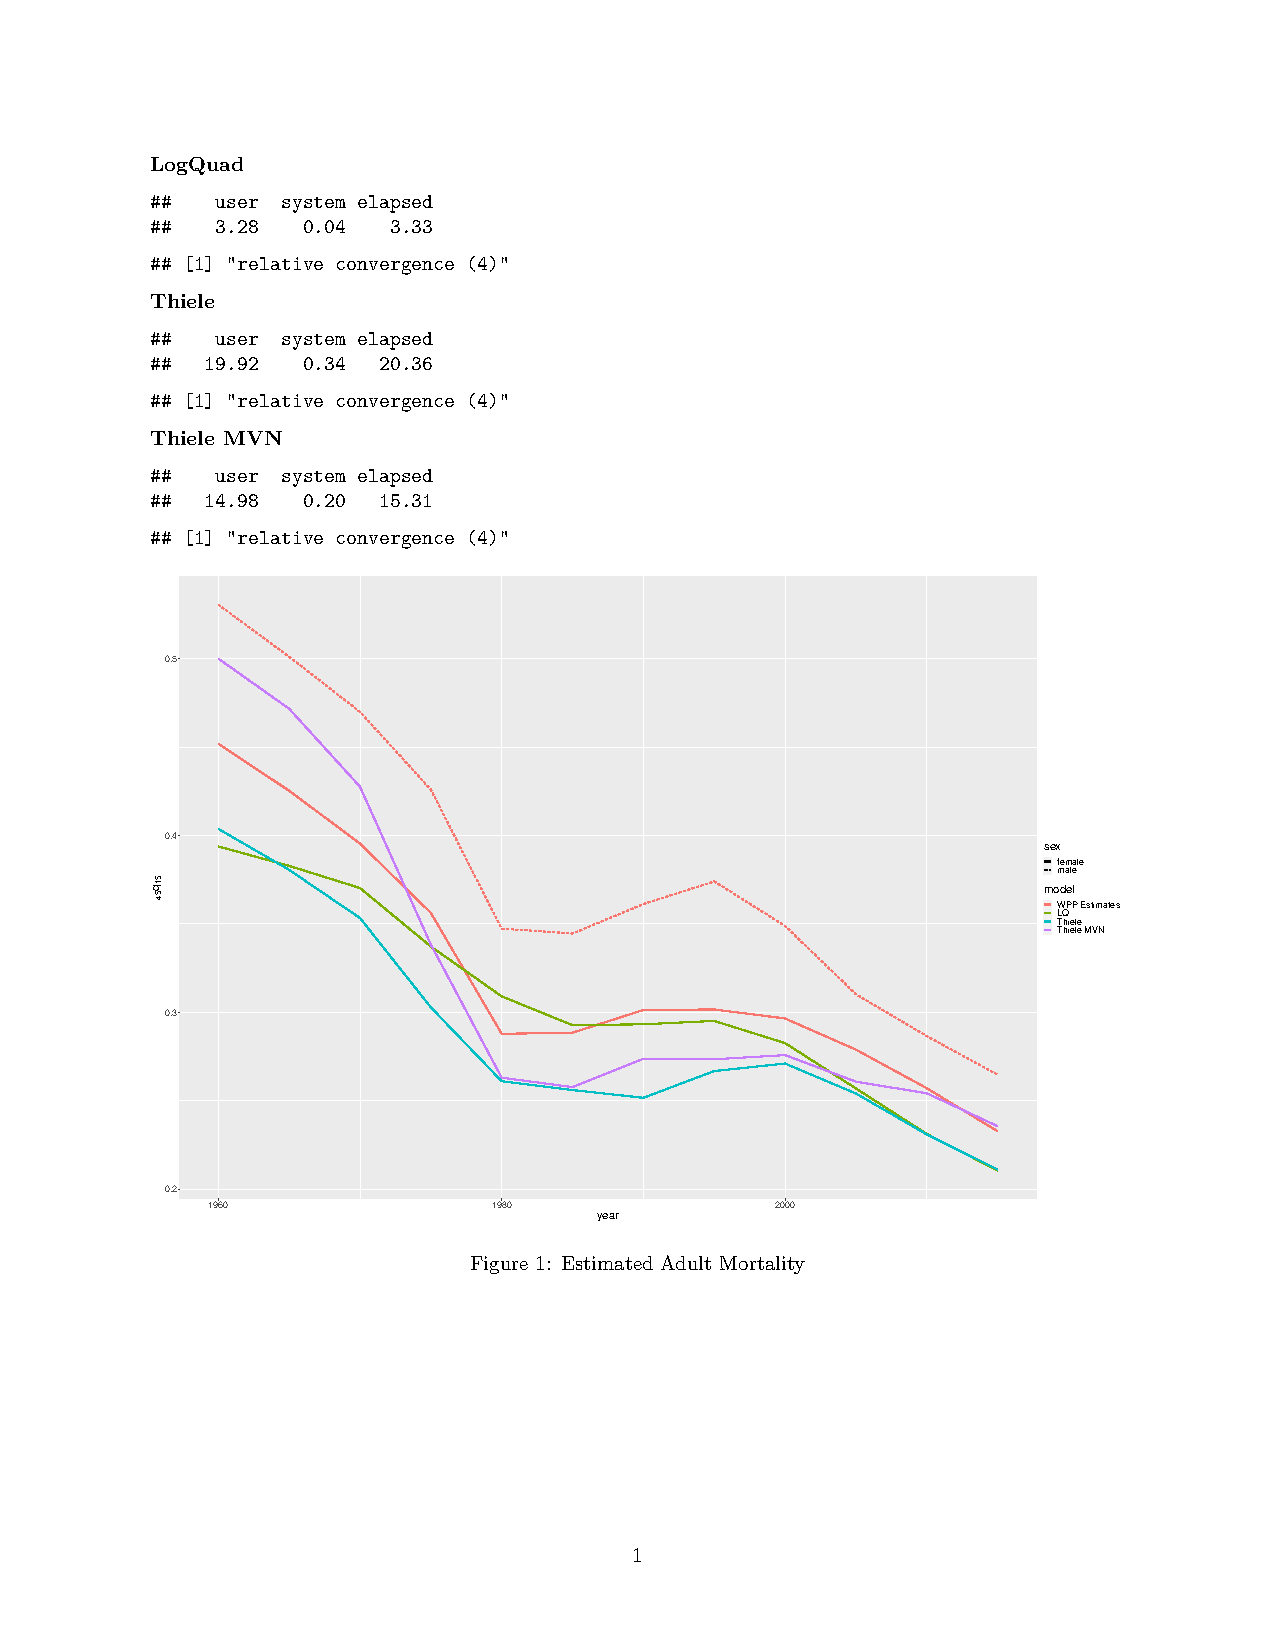
\includepdf[pages=-]{//BF.pdf}

\end{document} 